Transformações de Legendre tem ampla aplicação e interpretação. Faremos uma breve dissertação de duas possíveis visualizações do processo. 

\section{Tangentes}

Uma primeira interpretação do processo representa uma mudança clara de variável a partir de tangentes de uma função de concavidade bem definida. Faremos 

\[
	y = f(x) \mapsto \psi(\rho) = f(x(\rho)) - \rho x(\rho)
\]

onde 

\[
	\rho \equiv \frac{y - f(x(\rho))}{x - x(\rho)} = \frac{\psi(\rho) - f(x(\rho))}{0 - x(\rho)}
\]


Que podemos visualizar

\begin{center}
	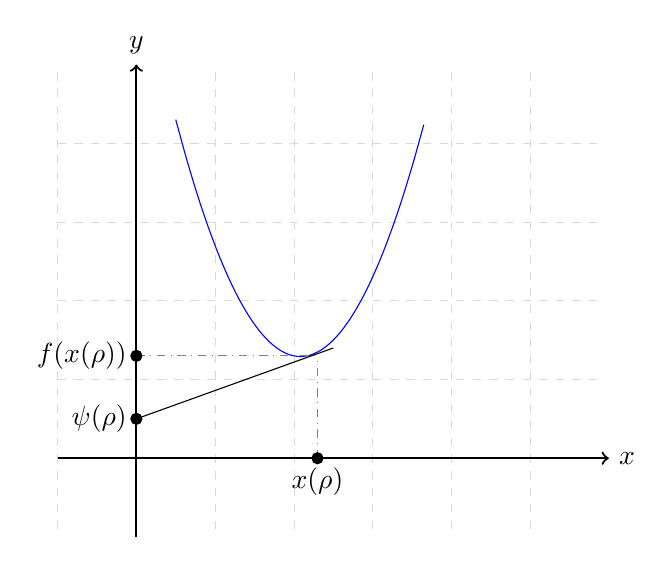
\begin{tikzpicture}[declare function={f(\x)=0.6*\x*\x - 5*\x + 13;}]
		\draw[help lines, color=gray!30, dashed] (-1,-0.9) grid (5.9,4.9);
		\draw[->,thick] (-1,0)--(6,0) node[right]{$x$};
		\draw[->,thick] (0,-1)--(0,5) node[above]{$y$};
		
		\draw[scale=0.5, domain=1:7.3, smooth, variable=\x, blue] plot ({\x}, {f(\x)});
		\draw (0,0.5) -- (2.5,1.4);
		\filldraw[black] (0,0.5) circle (2pt) node[anchor=east]{$\psi(\rho)$};
		\draw[gray, dash dot] (0,1.3) -- (2.3,1.3);
		\filldraw[black] (0,1.3) circle (2pt) node[anchor=east]{$f(x(\rho))$};
		\draw[gray, dash dot] (2.3,0) -- (2.3,1.3);
		\filldraw[black] (2.3,0) circle (2pt) node[anchor=north]{$x(\rho)$};
	\end{tikzpicture}
\end{center}

De forma que a transformada é criada pela projeção desta tangente no eixo x=0.


\section{Otimização}
Outra forma de visualizar a transformada é por um problema mais conveniente de otimização. Definiremos

\[
	\psi(\rho) = \max_x[\rho x - f(x)]
\]

Onde teremos

\begin{center}
	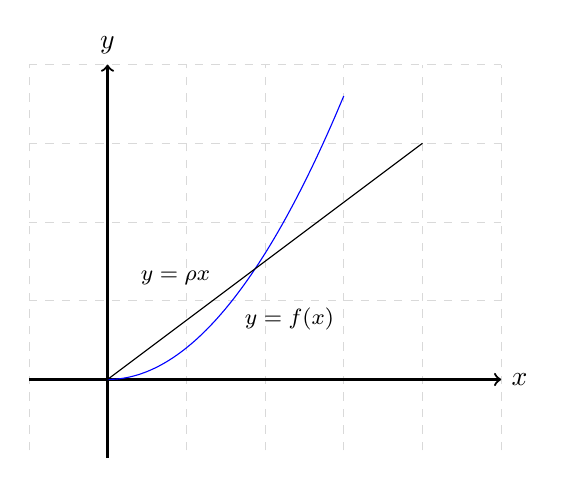
\begin{tikzpicture}[declare function={f(\x)=0.2*\x*\x;}]
		\draw[help lines, color=gray!30, dashed] (-1,-0.9) grid (5.0,4);
		\draw[->,thick] (-1,0)--(5,0) node[right]{$x$};
		\draw[->,thick] (0,-1)--(0,4) node[above]{$y$};
		
		\draw[scale=0.5, domain=0:6, smooth, variable=\x, blue] plot ({\x}, {f(\x)});
		\draw (0,0) -- (4,3);
		\node[above left] at (3.0,0.5) {\footnotesize $y=f(x)$};
		\node[below right] at (0.3,1.5) {\footnotesize $y=\rho x$};
	\end{tikzpicture}
\end{center}

Se definirmos 

\[
	g(x) = \rho x - f(x)
\]

Minimizaremos $g(x)$ e teremos a condição $f'(x^*) = \rho$. Ou seja

\[
	f'(x(\rho))=\rho \implies \max_x[\rho x - f(x)] = \rho x(\rho) - f(x(\rho))
\]

Que é equivalente à dizer

\[
\psi(\rho) = \min_x[f(x) - \rho x] = f(x(\rho)) - \rho x(\rho)
\]
